\documentclass[12pt]{article}                                                                                                                       
\usepackage{sbc-template}                                                 
\usepackage{graphicx,url}                                                 
\usepackage[utf8]{inputenc}                                               
\usepackage[brazil]{babel}                                                      
\usepackage{graphicx}

\title{Lista 3\\ Inteligência Artificial}
\author{Iyan Lucas Duarte Marques\inst{1}, Samir do Amorim Cambraia\inst{1}}

\address{Instituto de Ciências Exatas e Informática - Pontifícia Universidade Católica Minas Gerais (PUC-MG)}

\begin{document}

\maketitle

\section{Questão 01\\
  Faça um resumo do artigo “Estudo Comparativo entre os algoritmos de Mineração de Dados Random Forest e J48 na tomada de Decisão” que está no CANVAS
 }
O artigo apresenta uma comparação dos métodos de \textit{data mining} J48 e Random Forest utilizando como base os dados de óbitos do Rio Grande do Sul de 2013 (30 mil linhas).
Após uma breve introdução de ambos algoritmos e da base em si, o autor apresenta os resultados da comparação que se resume em:
\begin{itemize}
	\item \textbf{\textit{J48:}} Apresenta tempo de execução \textit{de facto} baixos, porém baixa taxa de acerto.
	\item \textbf{\textit{Random Forest:}} Apresenta altissima taxa de acerto ($\approx 99.7\%$), entretanto possui um alto tempo de execução.
\end{itemize}

\section{Questão 02\\
  Faça um resumo do artigo “Balanceamento de Dados” que está no CANVAS
 }
O artigo, \textit{A Study of Behavior of Several Methods for Balancing Machine Learning Training Data} apresenta o conceito de um dos maiores problemas do Machine Learning: o desbalanceamento de classes.
Desta forma, classes não balanceadas se tornam grandes empecilhos, principalmente para algoritmos de classificação.
Como solução, o artigo propõe a comparação entre vários métodos de balanceamento.
Sucintamente, os métodos podem ser divididos entre métodos de oversampling e undersampling.
Contrariando a opinião geral da comunidade que pesquisa ML, o artigo conclui que, os métodos de oversampling, foram mais eficientes em auxiliar a indução de classificadores, além de contribuir para o aumento de acurácia dos métodos, em contrapartida dos metodos de undersampling, que foram inferiores nestes quesitos.

\section{Questão 03\\
  Cite e explique os principais parâmetros que podem ser ajustados para melhorar o desempenho do classificador Random Forest.
  Quais os valores default destes parâmetros na ferramenta WEKA?.
  Explique cada um deles.
  Investigue o funcionamento do algoritmo no Python
 }

\begin{itemize}
	\item \textbf{\textit{Delimitar a profundidade máxima das árvores:}}
	      Por padrão, as árvores são expandidas até que todas as folhas sejam puras ou contenham menos do que as amostras mínimas para a divisão.
	      Isso ainda pode fazer com que as árvores se ajustem demais ou mal.
	      Desta forma, achar o numero ótimo de profundidade também torna o método mais eficiente
	\item \textbf{\textit{Aumentar ou diminuir o número de estimadores:}}
	      Maior numero de estimadores, maior a acurácia.
	      Menor numero de estimadores, maior a velocidade
	\item \textbf{\textit{Especificar o numero máximo de features a serem incluidas em cada split:}}
	      Isso depende muito do seu conjunto de dados.
	      Se suas variáveis independentes forem altamente correlacionadas, você desejará diminuir o número máximo de recursos.
	      Se seus atributos de entrada não estiverem correlacionados e seu modelo estiver sofrendo de baixa precisão, aumente o número de recursos a serem incluídos.
\end{itemize}
Utilizando a ferramenta WEKA, o método Random Forest possui os seguintes valores por \textit{default:}
\begin{figure}[h]
	\centering
	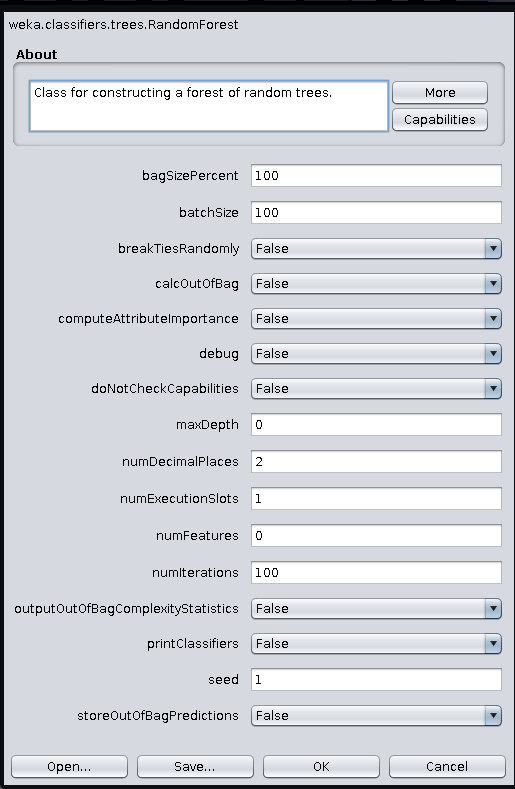
\includegraphics[width = 0.75\textwidth]{ibagens/atributos_weka.png}
\end{figure}

\begin{itemize}
	\item \textbf{\textit{bagSizePercent:}}
	      Size of each bag, as a percentage of the training set size. (default 100)
	\item \textbf{\textit{batchSize:}}
	      The desired batch size for batch prediction  (default 100).
	\item \textbf{\textit{breakTreeRandomly:}}
	      Break ties randomly when several attributes look equally good.
	\item \textbf{\textit{calcOutOfBag:}}
	\item \textbf{\textit{computeAtributeImportance:}}
	      Compute and output attribute importance (mean impurity decrease method)
	\item \textbf{\textit{debug:}}
	      If set, classifier is run in debug mode and may output additional info to the console
	\item \textbf{\textit{doNotCheckCapabillities:}}
	      If set, classifier capabilities are not checked before classifier is built
	      (use with caution).
	\item \textbf{\textit{maxDepth:}}
	      The maximum depth of the tree, 0 for unlimited.
	      (default 0)
	\item \textbf{\textit{numDecimalPlaces:}}
	      The number of decimal places for the output of numbers in the model (default 2).
	\item \textbf{\textit{numExecutionSlots:}}
	      Number of execution slots.
	      (default 1 - i.e. no parallelism)
	      (use 0 to auto-detect number of cores)
	\item \textbf{\textit{numFeatures:}}
	      Number of attributes to randomly investigate. (default 0)\\
	      $(<1 = int(log_2(\#predictors)+1))$.
	\item \textbf{\textit{numIterations:}}
	      Number of iterations (i.e., the number of trees in the random forest). (current value 100)
	\item \textbf{\textit{outputOutOfBagComplexityStatistics:}}
	      Whether to output complexity-based statistics when out-of-bag evaluation is performed.
	\item \textbf{\textit{printClassifiers:}}
	      Print the individual classifiers in the output
	\item \textbf{\textit{seed:}}
	      Seed for random number generator.
	      (default 1)
	\item \textbf{\textit{storeOutOfBagPredictions:}}
	      Whether to store out of bag predictions in internal evaluation object.
\end{itemize}

O algoritmo em python pode ser na biblioteca sklearn.
\section{Questão 04\\
  Faça um resumo comparativo entre os seguintes métodos do tipo ensemble
 }
\subsection{Bagging}
No Bagging os classificadores são treinados de forma independente por diferentes conjuntos de treinamento através do método de inicialização.
Para construí-los é necessário montar k conjuntos de treinamento idênticos e replicar esses dados de treinamento de forma aleatória para construir k redes independentes por re-amostragem com reposição.
Em seguida, deve-se agregar as k redes através de um método de combinação apropriada, tal como a maioria de votos (Breiman, 1996).

Para garantir que há amostras de treinamento suficientes em cada subconjunto, grandes porções de amostras (75-100\%) são colocadas em cada subconjunto.
Com isso, os subconjuntos individuais de formação se sobrepõem de forma significativa, com muitos casos fazendo parte da maioria dos subconjuntos e podendo até mesmo aparecer várias vezes num mesmo subconjunto.
A fim de assegurar a diversidade de situações, um learner de base relativamente instável é usado para que limites de decisão diferentes possam ser obtidos, considerando-se pequenas perturbações em diferentes amostras de treinamento (Wang, 2011).

\subsection{Boosting}
No Boosting, de forma semelhante ao Bagging, cada classificador é treinado usando um conjunto de treinamento diferente.
A abordagem por Boosting original foi proposta por Schapire em 1990.
A principal diferença em relação ao Bagging é que os conjuntos de dados re-amostrados são construídos especificamente para gerar aprendizados complementares e a importância do voto é ponderado com base no desempenho de cada modelo, em vez da atribuição de mesmo peso para todos os votos.
Essencialmente, esse procedimento permite aumentar o desempenho de um limiar arbitrário simplesmente adicionando learners mais fracos.
Dada a utilidade desse achado, Boosting é considerado uma das descobertas mais significativas em aprendizado de máquina (LANTZ, 2013).

\subsection{Random Forest}
Uma Random Forest é uma técnica de aprendizado de máquina usada para resolver problemas de regressão e classificação.
Ele utiliza aprendizagem por conjunto, que é uma técnica que combina muitos classificadores para fornecer soluções para problemas complexos.

Um algoritmo de random forest consiste em muitas árvores de decisão.
A "floresta" gerada pelo RF é treinada por meio de bagging ou bootstrap agregation.

O algoritmo estabelece o resultado com base nas previsões das árvores de decisão.
Ele prevê tomando a média ou média da produção de várias árvores.
Aumentar o número de árvores aumenta a precisão do resultado.

Uma RF erradica as limitações de um algoritmo de árvore de decisão.
Reduz o overfitting de conjuntos de dados e aumenta a precisão.


\section{Questão 05\\
  Considerando a base de dados “Breast Cancer.arff”(que está no CANVAS)experimente um(1) algoritmo de balanceamento undersampling e um(1)oversampling.
  Compare os resultados com a base de dados desbalanceada.
  Discuta os resultados.
  Você pode utilizar qualquer algoritmo de aprendizado (árvore, random forest, etc).
 }

Ambos tiveram o mesmo resultado.


\section{Questão 06\\
  A partir das matrizes de confusão obtidas na questão acima, calcule as métricas TVP, TVN, TFP, TFN, recall, precisão e F-measure.
 }

\begin{center}
	\begin{tabular}{| r | l | l | l | l | l | l | l |}
		\hline
		\textbf{TVP} & \textbf{TNP} & \textbf{TFP} & \textbf{TFN} & \textbf{Recall} & \textbf{Precisão} & \textbf{F1Score} \\ \hline
		0,696        & 0,304        & 0,543        & 0,304        & 0,696           & 0,664             & 0,669            \\ \hline
	\end{tabular}
\end{center}


\end{document}
